\section{Aufgabe 4.1}
\subsection{Berechnung der Fehlerrate}
In diesem Aufabenteil sollte ein Hopfield Modell mit 100 Neuronen implementiert werden. In Abhängigkeit von $p/N = 0.1, 0.2, 0.3$ sollte die Fehlerraten nach einer Iteration und nach Erreichen des Fixpunktes berechnet werden, indem man einmal von jedem exakten Bild startet. Dies wurde sowohl für ein asynchrones als auch für ein synchrones Update durchgeführt. Um ein statistisch aussagekräftigere Fehlerate zu berechnen, wurden dabei für jedes $p/N$ 1000 Sets zufällige Bildern gewählt und daraus der Mittelwert bestimmt. In \autoref{fig:fehlerrate} sind die Fehlerraten in Abhängigkeit von $p/N$ dargestellt.

\begin{figure}[htp]
	\centering
	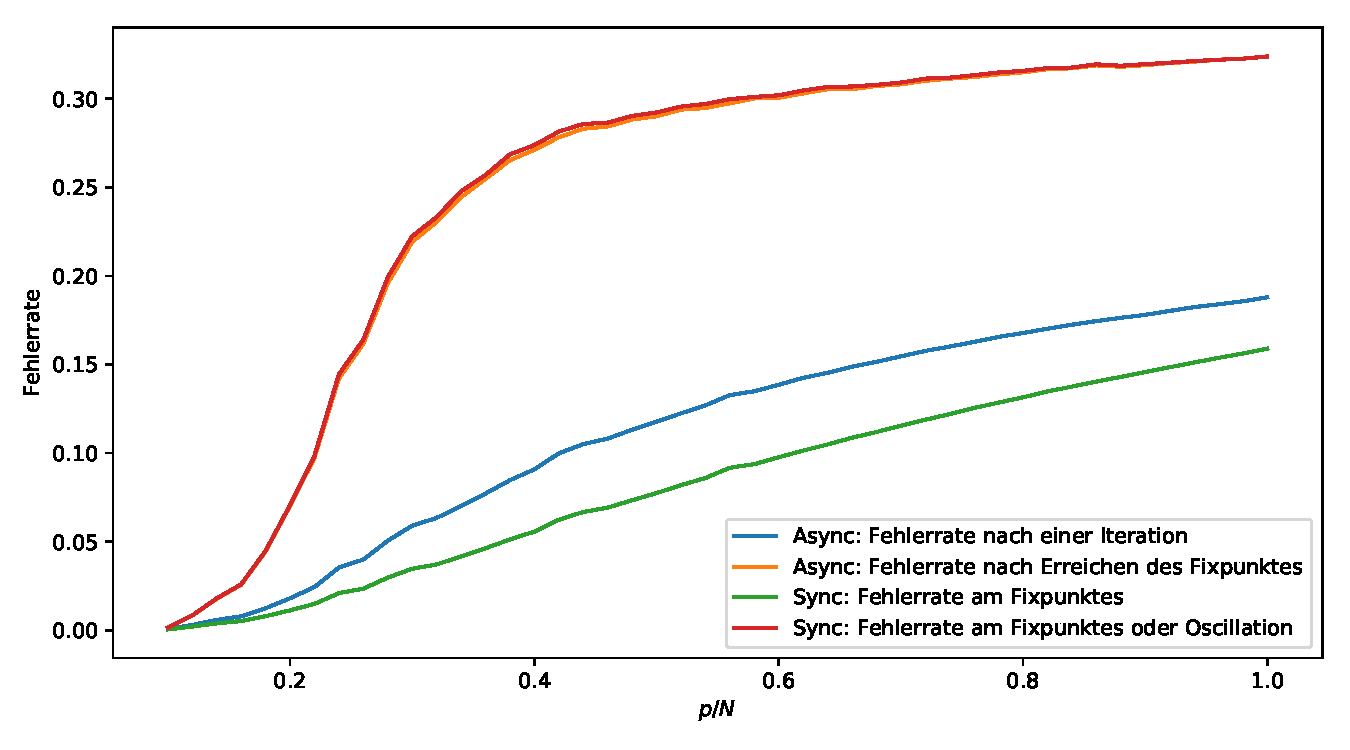
\includegraphics[width = \textwidth]{images/4_1/fehlerrate_1000.pdf}
	\caption{Die Fehlerrate in Abhängigkeit von $p / N = 0.1 \dots 1.0$. Hierbei wurde einmal ein asynchrones Update und einmal ein synchrones Update gewählt und der Fehler sowohl nach einer Iteration als auch nach Erreichen eines Fixpunktes (bei synchronen Update auch nach Erreichen einer Oszillation) dargestellt. Dabei wurden für jedes $p/N$ zufällige Sets von Bildern gewählt und der Mittelwert bestimmt.}
	\label{fig:fehlerrate}
\end{figure}

\noindent Es ist zu sehen, dass mit zunehhmenden $p/N$ die Fehlerrate des asynchronen und synchronen Updates sowohl nach einer Iteration als nach Erreichen des Fixpunktes zunimmt. Dies war zu erwarten, da mit Anzahl der Bilder auch die Anzahl der Nebenminima steigt. Auffällig ist außerdem, dass die Fehlerrate ab $p/N = 0.3$ für das asynchrone Update nach einer Iteration etwa 5 Prozent über der des synchronen Updates liegt. 

Die Fehlerrate nach Erreichen eines Fixpunktes (bei synchronen Update auch nach Erreichen einer Oszillation) steigt für beide Update Modi von $0.2 < p/N < 0.3$ etwa linear an und konvergiert dann bei $p/N = 1.0$ gegen 0.35. Es ist außerdem zu sehen, dass die Fehlerrate des synchronen Updates nach Erreichen des Fixpunktes im Bereich $0.2 < p/N < 0.3$ minimal unter der des asynchronen Updates liegt. Die Ursache dafür konnte bei den eintretenden Oszillationen liegen, aber könnte auch an nicht auszureichender Statsitik liegen.

Außerdem wurde geprüft wie sich die Anzahl der Iterationen bis zum Erreichen eines Fixpunktes (bei synchronen Update auch nach Erreichen einer Oszillation) mit $p/N$ ändert. Der Zusammenhang ist in \autoref{fig:iterationen_fixpunkt} geplotted. 

\begin{figure}[htp]
	\centering
	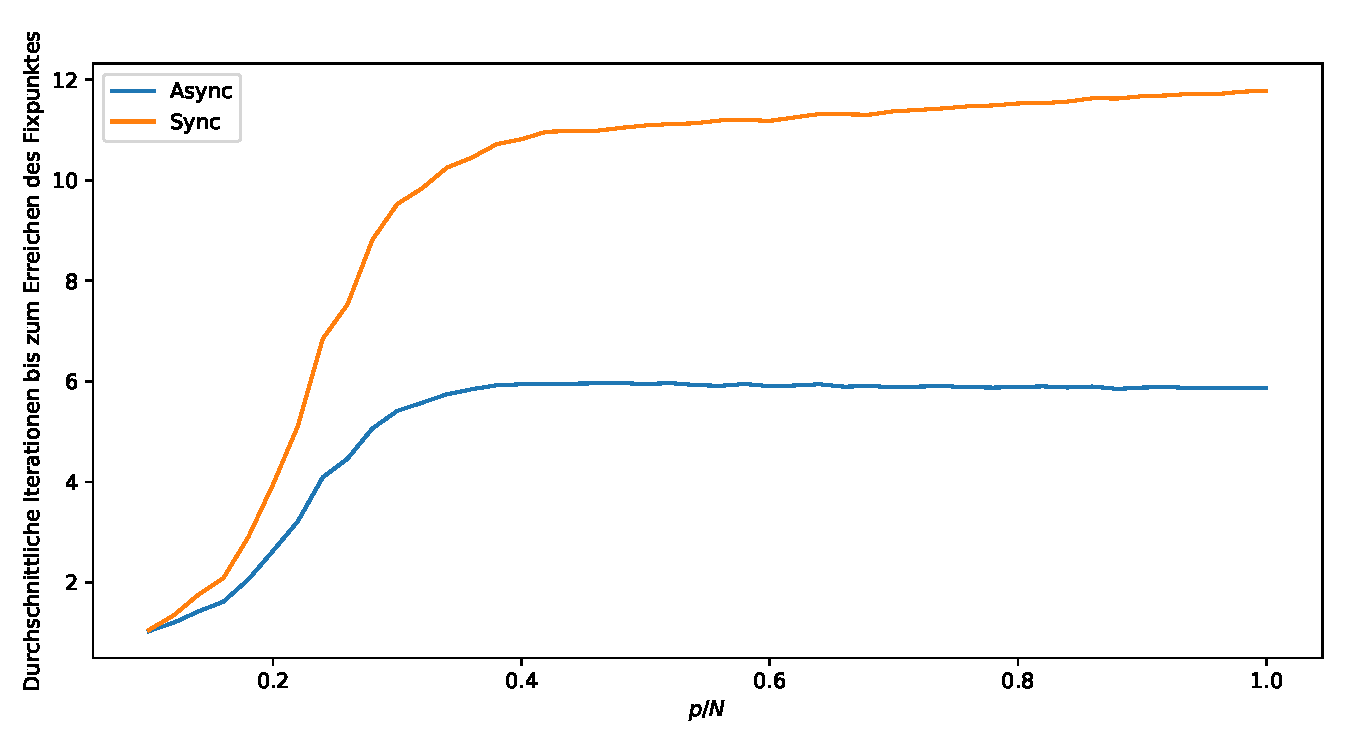
\includegraphics[width = \textwidth]{images/4_1/iterationen_fixpunkt_1000.pdf}
	\caption{Die Anzahl der benötigten Iterationen zum Erreichen eines Fixpunktes (bei synchronen Update auch nach Erreichen einer Oszillation) in Abhängigkeit von $p / N = 0.1 \dots 1.0$.}
	\label{fig:iterationen_fixpunkt}
\end{figure}

Auch hier nimmt die Anzahl der Iterationen bis zum Erreichen des Fixpunktes/Oszillation wie erwartet zu. Zu erkennen ist, dass die durchschnittlichen Iterationen bis zum Erreichen eines Fixpunktes/Oszillation beim synchronen Update deutlich größer sind als beim asynchronen Modus. Auch dies war zu erwarten, da im synchronen Modus mehrere Neuronen  gleichzeitig "denken" können, dass Sie durch ihre Änderung die Energie minimiert wird, aber es zu ein tatsächlich größeren Energie kommt. Im asynchronen Modus ist hingegen sichergestellt, dass jede Änderung zu einer Minimierung der Energiefunktion führt. Genauers dazu im folgenden \autoref{ssec:synchronesupdate}.


\subsection{Synchrones Update} \label{ssec:synchronesupdate}
Nun sollte erklärt werden, was sich bei dem synchronen Update ändert: Der wesentliche Unterschied zum asynchronen Update ist, wie der Name schon sagt, dass die Neuronen synchron aktualisiert werden. Dies kann im Unterschied zum asynchronen Update (hier werden die Neuronen nacheinander aktualisiert) zu einer Oszillation der Neuronen führen, was am folgenden Beispiel verdeutlicht werden soll (siehe \autoref{fig:2_neuron_hopfield_network}): 

\begin{figure}[htp]
	\centering
	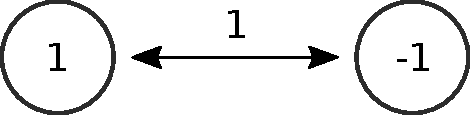
\includegraphics[width = 0.4\textwidth]{images/2_neuron_hopfield_network.pdf}
	\caption{Hopfield Netz aus 2 Neuronen. Im synchronen Modus wird hier keine Konvergenz erreicht: Die Neuronen oszillieren unendlich lange mit der Periode 2.}
	\label{fig:2_neuron_hopfield_network}
\end{figure}

Wir betrachten ein Netzwerk aus zwei Neuronen mit der Synapsen-Matrix $w_{12} = w_{21} = 1$ . Wird das Netz asynchron aktualisiert, so wird einer der  beiden stabilen Fixpunkte $(1,1)$ und $(-1,-1)$ erreicht. Im synchronen Modus sind diese Fixpunkte zwar auch stabil, allerdings besitzen diese kein "basis of attraction". Startet das Netzwerk synchron im Zustand $(1,-1)$ und $(-1,1)$ führt dies dazu, dass beide Neuronen die Energiefunktion gleichzeitig minimieren ''wollen'', aber es zu einem effektiven Anstieg der Energie kommt. Die Neuronen ''flippen'' ihr Vorzeichen und es kommt zu einer Unendlichen Oszillation. Diese Oszillationen besitzen dabei immer die Periode 2.

Dies ist auch nochmal für ein Hopfield Netzwerk im 4 Neuronen simuliert worden und ist in \autoref{fig:sync_oscillation} dargestellt:

\begin{figure}[htp]
	\centering
	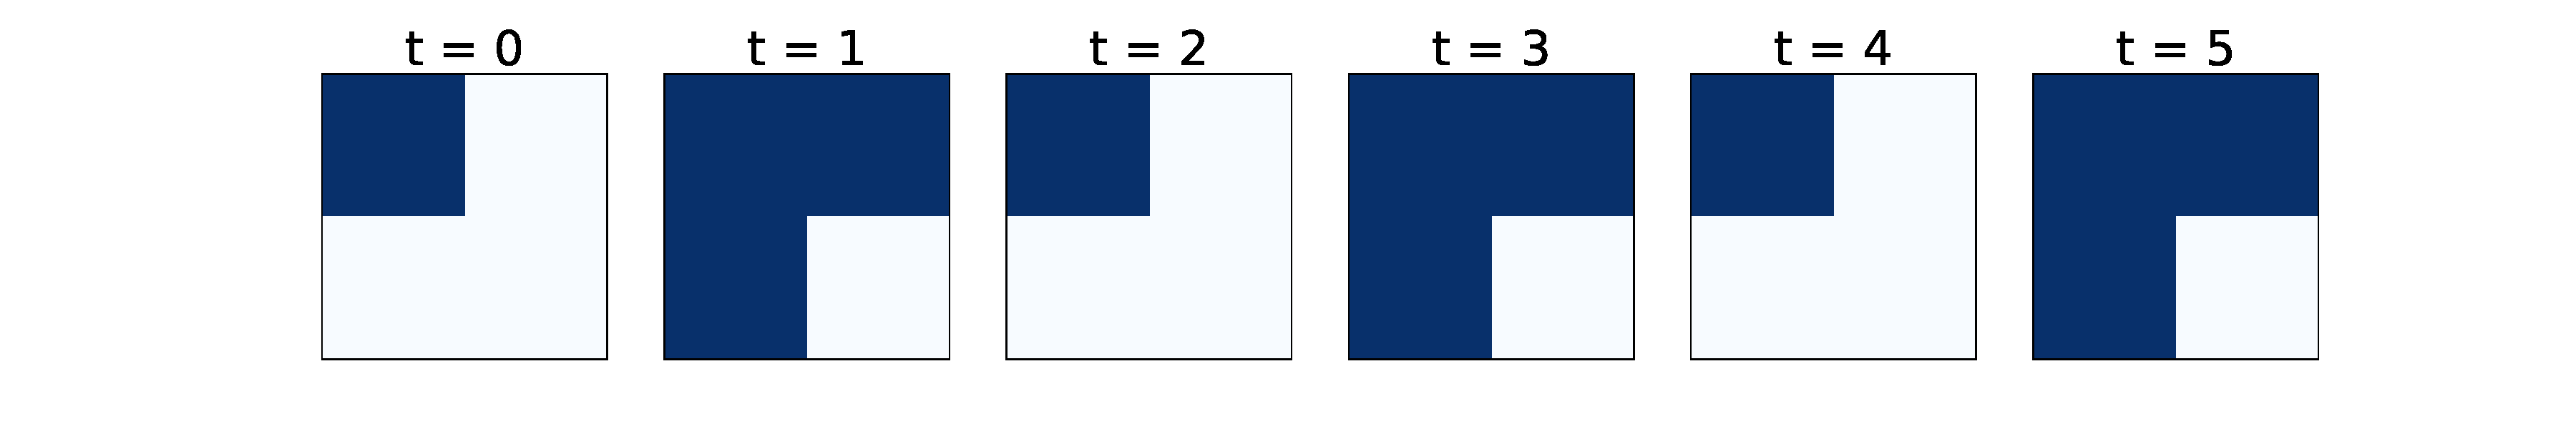
\includegraphics[width = \textwidth]{images/sync_oscillation.pdf}
	\caption{Hopfield Netz aus 4 Neuronen mit den trainierten Zuständen $(1,1,-1,-1)$ und $(1,-1,1,-1)$. Im synchronen Modus wird hier keine Konvergenz erreicht: Die Neuronen oszillieren unendlich lange mit der Periode 2.}
	\label{fig:sync_oscillation}
\end{figure}

Der Code zu Aufgabe 4.1 befindet sich in \textbf{aufgabe4\_1.py}.


\clearpage